\section{Linear parameter estimation} 
\label{LinParamEst}

%As can be seen in \eqref{multistate model_smallsignal}, the small signal model of such a multi-state/ multi-input system consists of two Jacobian matrices, one for the states and one for the inputs to the system. It should be emphasized however that these matrices have to be evaluated at the operating points, at $(\bar{x}, \bar{u})$. It is a reasonable statement since the inputs to the model are the small signal values of OD and differential pressures, dp, from the pumps. Therefore the same excitation to the real test setup can be carried out by taking the operating values into account and by adding them to the small signal values. 

The method that describes the linear parameter estimation is shown in \figref{fig:parame_block_lin} below:

\begin{figure}[H]
\centering
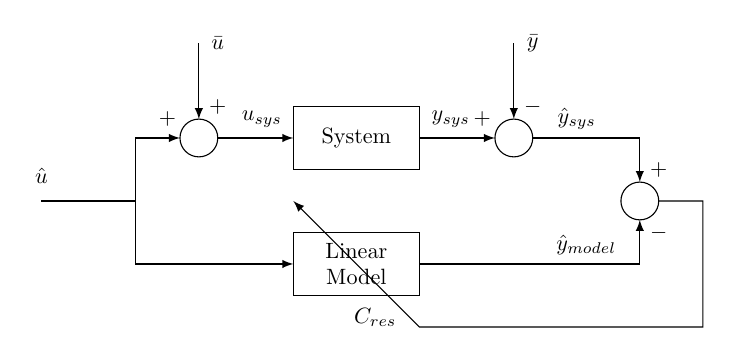
\begin{tikzpicture} [scale=0.8,transform shape]

\draw  (3,-1.5) rectangle (5,-2.5);
\node at (4,-1.8) {Linear};
\node at (4,-2.2) {Model};

\draw  (3,0.5) rectangle (5,-0.5);
\node at (4,0) {System};

\node at (8.8,-1.5) {$-$};
\node at (5.5,0.3) {$y_{sys}$};
\node at (7.5,0.3) {$\hat{y}_{sys}$};
\node at (7.65,-1.7) {$\hat{y}_{model}$};
\node at (4.3,-2.85) {$C_{res}$};
\node at (-1,-0.6) {$\hat{u}$};
\node at (1.8,1.5) {$\bar{u}$};
\node at (2.5,0.3) {$u_{sys}$};
\node at (8.8,-0.5) {$+$};
\node at (1.8,0.5) {$+$};
\node at (6,0.3) {$+$};
\node at (6.8,0.5) {$-$};
\node at (1,0.3) {$+$};
\node at (6.8,1.5) {$\bar{y}$};

\draw  (8.5,-1) ellipse (0.3 and 0.3);
\draw  (6.5,0) ellipse (0.3 and 0.3);
\draw  (1.5,0) ellipse (0.3 and 0.3);

\draw [-latex](5,0) -- (6.2,0);

\draw [-latex](0.5,-1) -- (0.5,0) -- (1.2,0);
\draw [-latex](0.5,-1) -- (0.5,-2) -- (3,-2);
\draw (-1,-1) -- (0.5,-1);
\draw [-latex](5,-2) -- (8.5,-2) -- (8.5,-1.3);
\draw [-latex](8.8,-1) -- (9.5,-1) -- (9.5,-3) -- (5,-3) -- (3,-1);

\draw [-latex](1.8,0) -- (3,0);
\draw [-latex](1.5,1.5) -- (1.5,0.3);
\draw [-latex](6.5,1.5) -- (6.5,0.3);
\draw [-latex](6.8,0) -- (8.5,0) -- (8.5,-0.7);
\end{tikzpicture}% 
\caption{Parameter identification block diagram for the linear system. }
\label{fig:parame_block_lin}
\end{figure}

In this case small-signal inputs are applied to both the test setup and the model.  Now the linearized model is compared to the real system, therefore the operating point is taken into account. Since the linear model is only valid for small deviations around the operating point, the real system has to be excited around the same operating point to obtain identical behavior. In order to achieve it, the operating values are added to both the input and the output such as: 

\begin{equation}
u_{sys} = \bar{u} + \hat{u}
 \label{u_smallsignal}
\end{equation}

\begin{minipage}[t]{0.20\textwidth}
Where\\
\hspace*{8mm} $\hat{u}$ \\
\hspace*{8mm} $\bar{u}$ \\
\hspace*{8mm} $u_{sys}$ 
\end{minipage}
\begin{minipage}[t]{0.68\textwidth}
\vspace*{2mm}
is the small-signal input, \\
is the operating value of the input,\\
is the input to the real-life system. 
\end{minipage}
\begin{minipage}[t]{0.10\textwidth}
\vspace*{2mm}
\textcolor{White}{te}$\unit{bar}$
\textcolor{White}{te}$\unit{bar}$
\textcolor{White}{te}$\unit{bar}$
\end{minipage} 

\begin{equation}
  y_{sys} = \bar{y} - \hat{y}_{sys} 
 \label{u_smallsignal}
\end{equation}

\begin{minipage}[t]{0.20\textwidth}
Where\\
\hspace*{8mm} $\hat{y}_{sys}$ \\
\hspace*{8mm} $\bar{u}_{sys}$ \\
\hspace*{8mm} $y_{sys}$ 
\end{minipage}
\begin{minipage}[t]{0.68\textwidth}
\vspace*{2mm}
is the small-signal output from the real-life system, \\
is the operating value of the output,\\
is the output from the real-life system. 
\end{minipage}
\begin{minipage}[t]{0.10\textwidth}
\vspace*{2mm}
\textcolor{White}{te}$\unit{bar}$
\textcolor{White}{te}$\unit{bar}$
\textcolor{White}{te}$\unit{bar}$
\end{minipage} 

During the linear parameter estimation, the same problem is solved as it is shown in \eqref{ObjectiveFunction}. In this case, however, the parameters are varied according to the comparison of the small-signal outputs.  

\subsection{Model Parameters}
\label{estimateParameters}
In order to obtain a complete model of the physical setup, all the parameters describing the components have to be defined. In \secref{SubSecEstimation} a detailed
description of the known parameters of the system has been done. Nevertheless, in the linearized state-space model more parameters have to be indentified
due to the introduction of the operating points values. Hence, in the current chapter a detailed compilation of the unknown parameters of the physical water distribution setup is carried out.


\subsection*{Unknown Parameters}
The unknown parameters are the ones related with the form losses, $k_f$, and form friction ,$f$, of the pipes. Despite they are 
provided by the manufactures they need to be estimated. On the one hand, the form losses depend on the fittings and bends of the pipes which they are not always known. 
On the other hand, the friction losses dependent on the inside average roughness of pipes, $\epsilon$, which can change its value due to passage of time 
and the rust generated inside pipes. 

%The friction and form losses are part of the model of a pipe, and are given by the following equation
%
%\begin{equation}
%  \lambda (q) =  \frac{8fL}{\pi^{2}gD^5} \rho g  |q| q + k_f \frac{8}{\pi^2gD^4} \rho g |q| q
%  \label{frictionestimation}
%\end{equation}

%From the above equation it can be seen that either estimating only for $k_f$ or $f$ will have the same result in the value of $\lambda (q)$.
%Therefore, it has been decided to carry out the estimation of the total value of $\lambda (q)$, hence discarding the respective values of $k_f$ and $f$.

Furthermore, the operating points of the flow through the chords, $\pmb{\bar{z}}$, is also unknown. These values, which correspond to the $8$ flow chords, are introduced in the linearized expression of both pipes 
and valves, see \eqref{lambda_lin} and \eqref{mu_lin}. Thus, not only pipe parameters introduce uncertainties into the system model but also the lack of knowledge of the chord operating points.

Consequently, it has been decided to estimate the total expression for the pressure across the pipes and valves in order to reduce the amount of unknowns in the system.

The system has $15$ pipes in total,  from \eqref{lambda_lin} it can be seen that either tunning for $k_f$, $f$ or $\pmb{\bar{z}}$ it will have the same result for the total
value of the pressure across the pipes, $\lambda(\pmb{{B_1^{T}}}\pmb{z})$. For this reason the pressure across the 15 pipes is estimated.

Valve linearized expression, see \eqref{mu_lin}, consists on the term depending on the chord flows and the one depending on the $OD$. Both terms include the operating 
point of the chord flows inside them, thus, the pressure difference given by both terms has to be estimated. In the system 4 valves take part, 
resulting in 8 unknowns in total. 

The WT connection edge, see \eqref{gamma_lin}, is conformed by two valves and one pump. Although the parameters corresponding to the pump are considered as known, the ones 
corresponding to the valves have to be estimated. Resulting in two more unknowns for the system. 

All in all, the system has $24$ unknown terms which will be calculated following the estimation process described in the next section.
\subsection{Measurements on the test setup}
\label{LinParamEst_measurements}

In order to verify the state-space model derived in \chapref{LinParamEst} with the physical setup, an estimation for the parameters defined in \secref{estimateParameters}
is carried out.

From the system setup $9$ different relative pressures can be measured, following \figref{systemdiagram} notation the sensors are placed in: 
$n_2$ $n_4$ $n_5$ $n_7$ $n_{10}$ $n_{11}$ $n_{15}$ $n_{16}$ $n_{18}$. However, the estimation will be done only the four PMA relative pressure 
sensor across the end-users and the pressure in the WT, since those are the outputs that will be controlled in \secref{SystemLin_control}. Thus, the estimation will be only focus on obtaining the best fit for those 
sensor outputs relevant in the control part. 

The relationship between pressures, where DpCXX describes the pressure difference for the XX component, is obtained in the same way as \secref{SubSecEstimation} and can be defined as:

\text{\underline{Node 10}}
\vspace{4mm}
\begin {equation}
     y_1 = DpC20 + DpC21  
\end{equation}

\text{\underline{Node 11}}
\vspace{4mm}
\begin {equation}
     y_2 = DpC24
\end{equation}


\text{\underline{Node 15}}
\vspace{4mm}
\begin {equation}
     y_3 = DpC28 + DpC20 
\end{equation}

\text{\underline{Node 15}}
\vspace{4mm}
\begin {equation}
     y_4 = DpC31 
\end{equation}

There is no need to define a relation with a referent point for the WT node, since the pressure across the WT is the state of the state-space model. 

\subsection{Estimation Data}

As the parameter estimation is based on a linearized model an operating point for the system is chosen. This point is based on the tank level being approximately half way full which allows for an equal amount of deviation in both directions. For the chosen operating point, data is gather from the system while small steps are individually applied to the two main pumps and the opening degree of the PMA valves. In order to use the data for parameter estimation the operating point is subtracted, leaving only small signal values.  

The operating point of the PMA valves is chosen to $63^{\circ}$ and the small signal values for the estimation can be seen in \figref{fig:est_OD_data}.

\begin{figure}[H]
\centering
% This file was created by matlab2tikz.
%
%The latest updates can be retrieved from
%  http://www.mathworks.com/matlabcentral/fileexchange/22022-matlab2tikz-matlab2tikz
%where you can also make suggestions and rate matlab2tikz.
%
\definecolor{mycolor1}{rgb}{0.00000,0.44700,0.74100}%
\definecolor{mycolor2}{rgb}{0.85000,0.32500,0.09800}%
\definecolor{mycolor3}{rgb}{0.92900,0.69400,0.12500}%
\definecolor{mycolor4}{rgb}{0.49400,0.18400,0.55600}%
%
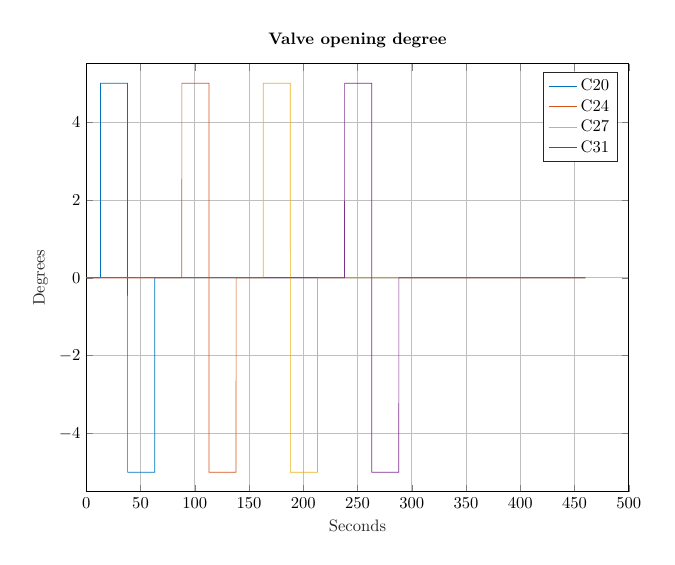
\begin{tikzpicture} [scale=0.6,transform shape]

\begin{axis}[%
width=4.521in,
height=3.566in,
at={(0.758in,0.481in)},
scale only axis,
xmin=0,
xmax=500,
xlabel style={font=\color{white!15!black}},
xlabel={Seconds},
ymin=-5.5,
ymax=5.5,
ylabel style={font=\color{white!15!black}},
ylabel={Degrees},
axis background/.style={fill=white},
title style={font=\bfseries},
title={Valve opening degree},
xmajorgrids,
ymajorgrids,
legend style={legend cell align=left, align=left, draw=white!15!black}
]
\addplot [color=mycolor1]
  table[row sep=crcr]{%
0	-1.13686837721616e-13\\
13.05	-1.13686837721616e-13\\
13.1	4.99999999999994\\
38.05	4.99999999999994\\
38.1	-5.00000000000006\\
63.05	-5.00000000000006\\
63.1	-1.13686837721616e-13\\
459.95	-1.13686837721616e-13\\
};
\addlegendentry{C20}

\addplot [color=mycolor2]
  table[row sep=crcr]{%
0	-1.13686837721616e-13\\
88.05	-1.13686837721616e-13\\
88.1	4.99999999999994\\
113.05	4.99999999999994\\
113.1	-5.00000000000006\\
138.05	-5.00000000000006\\
138.1	-1.13686837721616e-13\\
459.95	-1.13686837721616e-13\\
};
\addlegendentry{C24}

\addplot [color=mycolor3]
  table[row sep=crcr]{%
0	-1.13686837721616e-13\\
163.05	-1.13686837721616e-13\\
163.1	4.99999999999994\\
188.05	4.99999999999994\\
188.1	-5.00000000000006\\
213.05	-5.00000000000006\\
213.1	-1.13686837721616e-13\\
459.95	-1.13686837721616e-13\\
};
\addlegendentry{C27}

\addplot [color=mycolor4]
  table[row sep=crcr]{%
0	-1.13686837721616e-13\\
238.05	-1.13686837721616e-13\\
238.1	4.99999999999994\\
263.05	4.99999999999994\\
263.1	-5.00000000000006\\
288.05	-5.00000000000006\\
288.1	-1.13686837721616e-13\\
459.95	-1.13686837721616e-13\\
};
\addlegendentry{C31}

\end{axis}
\end{tikzpicture}% 
\caption{Small signal values of the opening degrees of the pma valves. }
\label{fig:est_OD_data}
\end{figure}

Furthermore the operating point for the pumps is chosen at a speed of $\omega = 0.4$, where the small signal values for the estimation are shown in \figref{fig:est_deltap_data}. 

\begin{figure}[H]
\centering
% This file was created by matlab2tikz.
%
%The latest updates can be retrieved from
%  http://www.mathworks.com/matlabcentral/fileexchange/22022-matlab2tikz-matlab2tikz
%where you can also make suggestions and rate matlab2tikz.
%
\definecolor{mycolor1}{rgb}{0.00000,0.44700,0.74100}%
\definecolor{mycolor2}{rgb}{0.85000,0.32500,0.09800}%
%
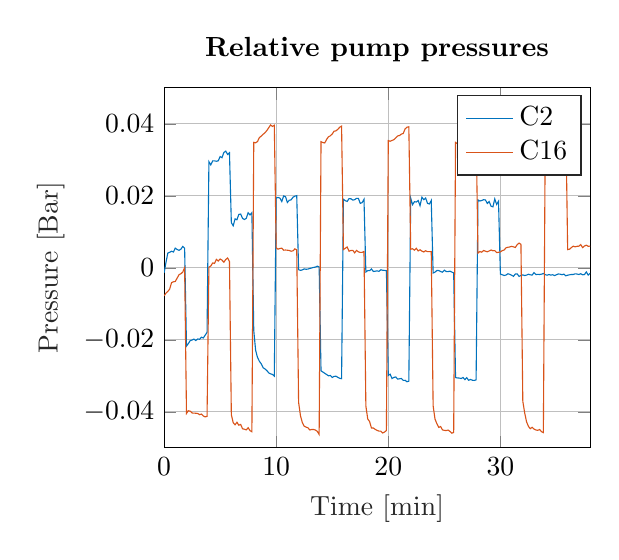
\begin{tikzpicture} 

\begin{axis}[%
scaled y ticks = false,
 y tick label style={/pgf/number format/fixed,
/pgf/number format/1000 sep = \thinspace}, % Optional if you want to replace comma as the 1000 separator 
width=2.13in,
height=1.8in,
at={(0.758in,0.481in)},
scale only axis,
xmin=0,
xmax=38,
xlabel style={font=\color{white!15!black}},
xlabel={Time [min]},
ymin=-0.05,
ymax=0.05,
ytick = {-0.04,-0.02,0,0.02,0.04},
ylabel style={font=\color{white!15!black}},
ylabel={Pressure [Bar]},
axis background/.style={fill=white},
title style={font=\bfseries},
title={Relative pump pressures},
xmajorgrids,
ymajorgrids,
legend style={legend cell align=left, align=left, draw=white!15!black}
]
\addplot [color=mycolor1]
  table[row sep=crcr]{%
0	-0.00139489180470775\\
0.166666666666664	0.00145823625003061\\
0.333333333333336	0.0041219703653752\\
0.5	0.00432358326860083\\
0.666666666666664	0.0046229478824884\\
0.833333333333336	0.00441522549733975\\
1	0.00548438483264846\\
1.16666666666666	0.00510559695385382\\
1.33333333333334	0.00487343664106987\\
1.5	0.00519112970069813\\
1.66666666666666	0.00597314338593691\\
1.83333333333334	0.00545994690499896\\
2	-0.0217211381389646\\
2.16666666666666	-0.0210185477186329\\
2.33333333333334	-0.0201937676599826\\
2.5	-0.0200349211301685\\
2.66666666666666	-0.0197844323717575\\
2.83333333333334	-0.0201876581782088\\
3	-0.0197355565164301\\
3.16666666666666	-0.0198394177090009\\
3.33333333333334	-0.0192590169269877\\
3.5	-0.0194789582759611\\
3.66666666666666	-0.0186786161449746\\
3.83333333333334	-0.0179332593512314\\
4	0.0295007582440334\\
4.16666666666666	0.028602664402392\\
4.33333333333334	0.029708480629175\\
4.5	0.0297206995930068\\
4.66666666666666	0.029622947882352\\
4.83333333333334	0.0297329185568387\\
5	0.0309242675304446\\
5.16666666666666	0.0306004649889005\\
5.33333333333334	0.0320545216851684\\
5.5	0.032439419045879\\
5.66666666666666	0.0315168872765739\\
5.83333333333334	0.0319873173841003\\
6	0.0125652743733653\\
6.16666666666666	0.0116916184593876\\
6.33333333333334	0.0136161052629049\\
6.5	0.0133717259862678\\
6.66666666666666	0.0148380016460905\\
6.83333333333334	0.0149540818024931\\
7	0.0137444043831394\\
7.16666666666666	0.0134328208054271\\
7.33333333333334	0.0137627328288872\\
7.5	0.015308431753617\\
7.66666666666666	0.0147035930439401\\
7.83333333333334	0.0153328696812807\\
8	-0.0174017344242614\\
8.16666666666666	-0.0228941586666807\\
8.33333333333334	-0.0248797402893572\\
8.5	-0.0259366806608128\\
8.66666666666666	-0.0266392710811445\\
8.83333333333334	-0.0277328683440956\\
9	-0.0280688898494716\\
9.16666666666666	-0.0285209915112503\\
9.33333333333334	-0.0291624871124228\\
9.5	-0.0294374137986395\\
9.66666666666666	-0.0296084792922855\\
9.83333333333334	-0.0300666904359801\\
10	0.0194201130830365\\
10.1666666666667	0.0195545216851869\\
10.3333333333333	0.0193834561915409\\
10.5	0.0184181580488243\\
10.6666666666667	0.0199821854193019\\
10.8333333333333	0.0197561345884125\\
11	0.0181676692902712\\
11.1666666666667	0.0187969459276118\\
11.3333333333333	0.0188885881563508\\
11.5	0.0196217259862621\\
11.6666666666667	0.0199149811182266\\
11.8333333333333	0.0200738276480408\\
12	-0.000490688480972779\\
12.1666666666667	-0.00069841086611433\\
12.3333333333333	-0.000564002263963914\\
12.5	-0.000276856613915299\\
12.6666666666667	-0.000392936770317931\\
12.8333333333333	-0.000325732469242723\\
13	-0.000142448011764884\\
13.1666666666667	-3.24773372781806e-05\\
13.3333333333333	0.000138588156367803\\
13.5	0.00020579245744301\\
13.6666666666667	0.000474609661743841\\
13.8333333333333	0.000285215722350074\\
14	-0.0286004147761574\\
14.6666666666667	-0.0299811576891571\\
14.8333333333333	-0.0298834059785023\\
15	-0.0304454783147676\\
15.1666666666667	-0.0301400042189712\\
15.3333333333333	-0.0300911283636438\\
15.5	-0.0304088214232721\\
15.6666666666667	-0.030671529145657\\
15.8333333333333	-0.0307814998201437\\
16	0.0190474346861649\\
16.1666666666667	0.0186625373254614\\
16.3333333333333	0.0184609244222358\\
16.5	0.0192368286255586\\
16.6666666666667	0.0192001717340631\\
16.8333333333333	0.0188152743733596\\
17	0.0189435734935941\\
17.1666666666667	0.0193101424085498\\
17.3333333333333	0.0192857044808861\\
17.5	0.0179110710498023\\
17.6666666666667	0.0181249029168598\\
17.8333333333333	0.019035215722333\\
18	-0.001150512527893\\
18.1666666666667	-0.000765615167189537\\
18.3333333333333	-0.000771724649105465\\
18.5	-0.000313513505410867\\
18.6666666666667	-0.000991665998078872\\
18.8333333333333	-0.00093668066083552\\
19	-0.000820600504432889\\
19.1666666666667	-0.00096722807041516\\
19.3333333333333	-0.000527345372468346\\
19.5	-0.000661753974618762\\
19.6666666666667	-0.00069841086611433\\
19.8333333333333	-0.000796162576769177\\
20	-0.0298895154604182\\
20.1666666666667	-0.0295351655092944\\
20.3333333333333	-0.0307448429286481\\
20.5	-0.0304210403871039\\
20.6666666666667	-0.0303049602307013\\
20.8333333333333	-0.0309036894584622\\
21.1666666666667	-0.0307265144830779\\
21.3333333333333	-0.0312641488921628\\
21.5	-0.031233601482441\\
21.6666666666667	-0.0316307178070971\\
21.8333333333333	-0.03146576179536\\
22	0.0193712372271335\\
22.1666666666667	0.0175628305800331\\
22.3333333333333	0.0183937201206206\\
22.5	0.018289858927929\\
22.6666666666667	0.018711413180192\\
22.8333333333333	0.0172695754479975\\
23	0.0196339449495255\\
23.1666666666667	0.0189435734929546\\
23.3333333333333	0.0193956751548825\\
23.5	0.0179171805310432\\
23.6666666666667	0.0177461150374967\\
23.8333333333333	0.0187053036983613\\
24	-0.00143765817838926\\
24.1666666666667	-0.00119327890195819\\
24.3333333333333	-0.000728958276326352\\
24.5	-0.000747286722067031\\
24.6666666666667	-0.00101610392621865\\
24.8333333333333	-0.0012116073475994\\
25	-0.000643425529389674\\
25.1666666666667	-0.0010161039262897\\
25.3333333333333	-0.00103443237210854\\
25.5	-0.00092446169750815\\
25.8333333333333	-0.00139489180502039\\
26	-0.0304821352068458\\
26.1666666666667	-0.0305737774356487\\
26.3333333333333	-0.0306104343272011\\
26.5	-0.0307326239654202\\
26.6666666666667	-0.0304454783153716\\
26.8333333333333	-0.0310319885793149\\
27	-0.0305065731345238\\
27.1666666666667	-0.0312336014824908\\
27.3333333333333	-0.0310014411697779\\
27.5	-0.0312152730367785\\
27.6666666666667	-0.0312702583739508\\
27.8333333333333	-0.0311114118442362\\
28	0.0188763691920002\\
28.1666666666667	0.0185831140599433\\
28.3333333333333	0.0187114131802417\\
28.5	0.0189435734931322\\
28.6666666666667	0.0188580407461743\\
28.8333333333333	0.0179049615673108\\
29	0.0184120485664536\\
29.1666666666667	0.0171290573639737\\
29.3333333333333	0.0169579918702851\\
29.5	0.0191635148419067\\
29.6666666666667	0.0176178159172053\\
29.8333333333333	0.0185036907950433\\
30	-0.00171869434679195\\
30.3333333333333	-0.0021097011892337\\
30.5	-0.00198751155090093\\
30.6666666666667	-0.00163927108179962\\
30.8333333333333	-0.00178589864775347\\
31	-0.00203638740624257\\
31.1666666666667	-0.00235408046590635\\
31.3333333333333	-0.00169425641899323\\
31.5	-0.00168203745517559\\
31.6666666666667	-0.00236018994774412\\
31.8333333333333	-0.00210359170736751\\
32	-0.00194474517746102\\
32.1666666666667	-0.0021341391168832\\
32.3333333333333	-0.00200583999667714\\
32.5	-0.00177367968388609\\
32.6666666666667	-0.00192030724985415\\
32.8333333333333	-0.00200583999672688\\
33	-0.00130935905831819\\
33.1666666666667	-0.00185921243073039\\
33.3333333333333	-0.00181033657548113\\
33.5	-0.00183477450305247\\
33.6666666666667	-0.0017553512381312\\
33.8333333333333	-0.00156595729870901\\
34	-0.00188365035842963\\
34.1666666666667	-0.0020363874062852\\
34.3333333333333	-0.00185921243069487\\
34.5	-0.00200583999665582\\
34.6666666666667	-0.0019141977679098\\
34.8333333333333	-0.00213413911680505\\
35.1666666666667	-0.00168814693694941\\
35.3333333333333	-0.00175535123805304\\
35.5	-0.00189586932216912\\
35.6666666666667	-0.00173702279234078\\
35.8333333333333	-0.0021952339360567\\
36	-0.00203638740630652\\
36.3333333333333	-0.00182866502116497\\
36.5	-0.00182866502110102\\
36.6666666666667	-0.00165149004562437\\
36.8333333333333	-0.00170647538281798\\
37	-0.00184088398482629\\
37.1666666666667	-0.00162705211794645\\
37.3333333333333	-0.00192030724991099\\
37.5	-0.00186532191253974\\
37.6666666666667	-0.00111996511879653\\
37.8333333333333	-0.00199362103295186\\
38	-0.00154762885295412\\
38.1666666666667	-0.00174924175630053\\
38.3333333333333	-0.00155984781689966\\
38.5	-0.00148042455182917\\
38.6666666666667	-0.0021707960084143\\
38.8333333333333	-0.00124215475717193\\
39	-0.00164538056368002\\
39.1666666666667	-0.00175535123807435\\
39.3333333333333	-0.00160261419026142\\
39.5	-0.00156595729870901\\
39.6666666666667	-0.00135823491364562\\
39.8333333333333	-0.00133379698605296\\
40	-0.00146209610613113\\
40.3333333333333	-0.00126659268493512\\
40.5	-0.00121771682960059\\
40.6666666666667	-0.00129103061253488\\
40.8333333333333	-0.000625097083712944\\
41	-0.00128492113057632\\
41.1666666666667	-0.00111996511900259\\
41.3333333333333	-0.00162705211793934\\
41.5	-0.000753396203876378\\
41.8333333333333	-0.000790053095428789\\
42	-0.000551783300679176\\
42.1666666666667	-0.000967228070969384\\
42.3333333333333	-0.000942790143270145\\
42.5	-5.69152657305949e-05\\
42.6666666666667	-0.000667863457231022\\
42.8333333333333	-0.000918352215485641\\
43	-0.000295185060139147\\
43.1666666666667	-0.000466250553920133\\
43.3333333333333	-8.03941040317113e-06\\
43.5	-0.00041737469859271\\
43.6666666666667	-0.000252418686997657\\
43.8333333333333	0.000150807119624119\\
44	0.000187464011091265\\
44.1666666666667	0.000859507021942818\\
44.5	0.000468500179252374\\
44.6666666666667	0.000841178576258983\\
44.8333333333333	0.000828959612164226\\
45	0.00100613458785404\\
45.1666666666667	0.000810631166686449\\
45.3333333333333	0.00114054319011103\\
45.6666666666667	0.00200808962211596\\
45.8333333333333	0.00186146205631132\\
46	0.00167206811648413\\
46.1666666666667	0.00215471718811955\\
46.3333333333333	0.00297949724677693\\
46.5	0.0030589205116982\\
46.6666666666667	0.00295505931924822\\
46.8333333333333	0.00329108082453899\\
47	0.00370041611274985\\
47.1666666666667	0.003920357461908\\
47.3333333333333	0.00446410135237585\\
47.5	0.00480623233950439\\
47.6666666666667	0.00554547965146668\\
47.8333333333333	0.00558824602479291\\
48	0.00607089509629333\\
48.1666666666667	0.00607700457781846\\
48.3333333333333	0.00632749333657046\\
48.5	0.00648023038446155\\
48.6666666666667	0.0064435734931152\\
48.8333333333333	0.00668184328783639\\
49	0.00712172598587557\\
49.1666666666667	0.00737221474435756\\
49.3333333333333	0.00696287945559959\\
49.5	0.00737221474424388\\
49.6666666666667	0.00789763018895684\\
49.8333333333333	0.00725613458760677\\
50	0.00776933106877209\\
50.1666666666667	0.00889347574166521\\
50.3333333333333	0.00866131542857573\\
50.5	0.0086613154285331\\
50.6666666666667	0.00889347574139521\\
50.8333333333333	0.00828252754984504\\
51	0.00849024993481606\\
51.1666666666667	0.00904621278917261\\
51.3333333333333	0.00888125677727913\\
51.5	0.00915007398194234\\
51.6666666666667	0.00991375922147597\\
51.8333333333333	0.00907676019874515\\
52	0.00919894983708502\\
52.1666666666667	0.00987099284792237\\
52.3333333333333	0.00940667222214842\\
52.5	0.00986488336603486\\
52.6666666666667	0.00959606616175535\\
52.8333333333333	0.00963272305312302\\
53	0.009370015330596\\
53.1666666666667	0.0100970436786199\\
};
\addlegendentry{C2}

\addplot [color=mycolor2]
  table[row sep=crcr]{%
0	-0.00779296760428139\\
0.166666666666664	-0.00701095391904261\\
0.333333333333336	-0.00655885225725683\\
0.5	-0.00589291872842779\\
0.666666666666664	-0.00410284052708221\\
0.833333333333336	-0.00387068021427694\\
1	-0.00377903798553803\\
1.33333333333334	-0.00190342703727708\\
1.5	-0.00164682879680811\\
1.66666666666666	-0.0011641797254498\\
1.83333333333334	5.16071758198677e-05\\
2	-0.0404481484450088\\
2.16666666666666	-0.0396844632055178\\
2.33333333333334	-0.0398127623257523\\
2.5	-0.0403137398428584\\
2.83333333333334	-0.0403809441439336\\
3	-0.0404481484450088\\
3.16666666666666	-0.040771950986553\\
3.33333333333334	-0.040600885492907\\
3.5	-0.0411568483472564\\
3.66666666666666	-0.0413951181419776\\
3.83333333333334	-0.0412423810940794\\
4	0.000198234741660031\\
4.16666666666666	0.000497599355540501\\
4.33333333333334	0.00137736475143413\\
4.5	0.00124295614928371\\
4.66666666666666	0.00235488185826682\\
4.83333333333334	0.00190888967840408\\
5	0.0024587430508376\\
5.16666666666666	0.00214715947312527\\
5.33333333333334	0.00157286817302804\\
5.5	0.00231822496677125\\
5.66666666666666	0.00274588870088621\\
5.83333333333334	0.00178059055816959\\
6	-0.0407780604681847\\
6.16666666666666	-0.0430019118855824\\
6.33333333333334	-0.0435884221495115\\
6.5	-0.0428858317291798\\
6.66666666666666	-0.0436983928239982\\
6.83333333333334	-0.0434967799207726\\
7	-0.0446942383762945\\
7.16666666666666	-0.0448164280146131\\
7.33333333333334	-0.0449997124720909\\
7.5	-0.04440098324433\\
7.66666666666666	-0.0452135443391484\\
7.83333333333334	-0.0455190184349448\\
8	0.0348512161690877\\
8.16666666666666	0.0347473549765169\\
8.33333333333334	0.035083376481893\\
8.5	0.03618308322676\\
8.66666666666666	0.0365985279970431\\
8.83333333333334	0.0371056149960651\\
9	0.0375271692482642\\
9.16666666666666	0.0381625553675207\\
9.33333333333334	0.0389140216431798\\
9.5	0.0397082542922504\\
9.66666666666666	0.0392989190038833\\
9.83333333333334	0.0396166120635115\\
10	0.00558068830987679\\
10.1666666666667	0.00519579094917333\\
10.3333333333333	0.0053851848885671\\
10.5	0.00548293659922194\\
10.6666666666667	0.00490864529912471\\
10.8333333333333	0.00495752115445214\\
11.1666666666667	0.00484144099804951\\
11.3333333333333	0.0046214996490761\\
11.5	0.00473757980547873\\
11.6666666666667	0.00526910473216446\\
11.8333333333333	0.00503083493744327\\
12	-0.0373384221495172\\
12.1666666666667	-0.0410652061182333\\
12.3333333333333	-0.0429835834398347\\
12.5	-0.0439794289921309\\
12.6666666666667	-0.0442360272325999\\
12.8333333333333	-0.0444193116900777\\
13	-0.0450363693635865\\
13.1666666666667	-0.0448958512795201\\
13.3333333333333	-0.0448958512795201\\
13.5	-0.0450485883274183\\
13.6666666666667	-0.0454090477604581\\
13.8333333333333	-0.0462765941925198\\
14	0.0350650480361452\\
14.1666666666667	0.0348084497956762\\
14.3333333333333	0.0347045886031054\\
14.5	0.0356943246734858\\
14.6666666666667	0.0364213530214812\\
14.8333333333333	0.0366840607438661\\
15	0.0371850382609722\\
15.1666666666667	0.037960942464295\\
15.3333333333333	0.0380586941749499\\
15.5	0.0384924673909808\\
15.6666666666667	0.039066758691078\\
15.8333333333333	0.0393722327868744\\
16	0.00509192975660255\\
16.3333333333333	0.00578841069501834\\
16.5	0.00463982809482388\\
16.6666666666667	0.00482311255230172\\
16.8333333333333	0.00486587892571322\\
17	0.00416939798729743\\
17.1666666666667	0.00484144099804951\\
17.3333333333333	0.00446265311926197\\
17.5	0.00428547814370006\\
17.6666666666667	0.00429158762561599\\
17.8333333333333	0.00456040482991682\\
18	-0.0383587056294772\\
18.1666666666667	-0.0419510809960428\\
18.3333333333333	-0.0427086567536179\\
18.5	-0.0444865159911529\\
18.6666666666667	-0.0444865159911529\\
18.8333333333333	-0.0448530849061086\\
19	-0.0451463400380732\\
19.1666666666667	-0.0453357339774669\\
19.3333333333333	-0.0453479529412988\\
19.5	-0.0458733683860686\\
19.6666666666667	-0.0456106606639182\\
19.8333333333333	-0.045170777966284\\
20	0.0353644126494927\\
20.1666666666667	0.0351750187100919\\
20.5	0.0356149014079747\\
20.8333333333333	0.0366535133336328\\
21	0.036763484008155\\
21.1666666666667	0.0371667098146276\\
21.3333333333333	0.0373194468625115\\
21.5	0.0386085475468576\\
21.6666666666667	0.0390728681723971\\
21.8333333333333	0.0391950578107299\\
22	0.00518357198486541\\
22.1666666666667	0.00530576162303475\\
22.3333333333333	0.00492086426232419\\
22.5	0.00543406074329766\\
22.6666666666667	0.00471314187723948\\
22.8333333333333	0.00503083493688194\\
23	0.00465204705809441\\
23.1666666666667	0.00441377726330927\\
23.3333333333333	0.00476812721451125\\
23.5	0.004499310010182\\
23.8333333333333	0.00449320052823765\\
24	-0.0383037202928449\\
24.1666666666667	-0.041999956852024\\
24.3333333333333	-0.043270729090402\\
24.5	-0.0443093410162447\\
24.6666666666667	-0.0440710712213814\\
24.8333333333333	-0.0449997124726593\\
25	-0.0451463400386771\\
25.1666666666667	-0.0451891064121241\\
25.3333333333333	-0.0450546978098814\\
25.5	-0.0454273762067956\\
25.6666666666667	-0.045916134760084\\
25.8333333333333	-0.045726740820669\\
26	0.0348573256503855\\
26.1666666666667	0.0345213041450236\\
26.3333333333333	0.0350833764813174\\
26.5	0.0352177850835247\\
26.6666666666667	0.0358287332751033\\
26.8333333333333	0.0360303461782649\\
27	0.0364885573219311\\
27.1666666666667	0.0365801995507482\\
27.3333333333333	0.0373622132360154\\
27.5	0.0380892415840108\\
27.6666666666667	0.0382786355233975\\
27.8333333333333	0.0383152924147865\\
28	0.00410830316747735\\
28.1666666666667	0.00454207638357218\\
28.3333333333333	0.00435268244412867\\
28.5	0.00482311255176171\\
28.8333333333333	0.00445654363672787\\
29.1666666666667	0.0049636306357641\\
29.3333333333333	0.00476201773265217\\
29.5	0.00480478410602103\\
29.6666666666667	0.00423660228762657\\
30	0.00442599622725481\\
30.1666666666667	0.00480478410603524\\
30.3333333333333	0.00494530219003764\\
30.5	0.00557457882741375\\
30.6666666666667	0.00572731587534037\\
30.8333333333333	0.00580062965826755\\
31	0.0059900235976329\\
31.3333333333333	0.00566622105601056\\
31.5	0.00646045370515225\\
31.6666666666667	0.00687589847543535\\
31.8333333333333	0.00652765800625588\\
32	-0.0370451670181851\\
32.1666666666667	-0.0402831924335416\\
32.3333333333333	-0.0427575326094498\\
32.5	-0.0440221953662459\\
32.6666666666667	-0.0446759099311222\\
32.8333333333333	-0.0442849030883963\\
33	-0.0447675521598754\\
33.1666666666667	-0.045024150400387\\
33.3333333333333	-0.0451402305566404\\
33.5	-0.0448836323163277\\
33.6666666666667	-0.045512908953576\\
33.8333333333333	-0.0457572882302912\\
34	0.0355415876250049\\
34.1666666666667	0.0355049307336017\\
34.3333333333333	0.0363908056113331\\
34.5	0.0368245788273924\\
34.6666666666667	0.0377348916328941\\
34.8333333333333	0.0374966218381445\\
35	0.0383030734510257\\
35.3333333333333	0.0389873354254959\\
35.5	0.0400015094236679\\
35.8333333333333	0.0410034644579085\\
36	0.00507360131026502\\
36.1666666666667	0.00518968146665344\\
36.3333333333333	0.00563567364651618\\
36.5	0.00603889945294611\\
36.6666666666667	0.00584339603171458\\
36.8333333333333	0.00599002359772527\\
37	0.00602668048919242\\
37.1666666666667	0.00647267266904095\\
37.3333333333333	0.00563567364648776\\
37.5	0.00607555634453405\\
37.6666666666667	0.00630771665723984\\
37.8333333333333	0.00599613307956304\\
38	0.00604500893485493\\
38.1666666666667	0.00551959349019882\\
38.3333333333333	0.00608166582632208\\
38.5	0.00620385546475433\\
38.6666666666667	0.0059106003326832\\
38.8333333333333	0.00583728654979865\\
39	0.00536074696035627\\
39.1666666666667	0.00616108909131441\\
39.3333333333333	0.00611221323602962\\
39.5	0.00600835204337358\\
39.6666666666667	0.00610610375406395\\
39.8333333333333	0.00603278997111545\\
40	0.0056723305382107\\
40.1666666666667	0.00588005292322435\\
40.3333333333333	0.00626495028393492\\
40.5	0.00607555634439905\\
40.6666666666667	0.00633826406681948\\
40.8333333333333	0.00611832271790291\\
41	0.00652154852429732\\
41.1666666666667	0.00677203728296405\\
41.5	0.00577619173058963\\
41.6666666666667	0.0067109424641103\\
41.8333333333333	0.00570287794787561\\
42	0.00650322007854953\\
42.1666666666667	0.00656431489780829\\
42.3333333333333	0.00642379681380589\\
42.5	0.00656431489805698\\
42.6666666666667	0.00653376748818602\\
42.8333333333333	0.00602057100731912\\
43	0.00631382613914866\\
43.1666666666667	0.00608166582653524\\
43.3333333333333	0.005776191730547\\
43.5	0.00626495028388518\\
43.6666666666667	0.00639324940434705\\
43.8333333333333	0.00628327872952639\\
44	0.00598391411572408\\
44.1666666666667	0.0058556149956317\\
44.3333333333333	0.00618552701919128\\
44.5	0.00625884080206873\\
44.6666666666667	0.00590449085063938\\
44.8333333333333	0.00646045370494619\\
45	0.00630160717548733\\
45.1666666666667	0.00647878215097109\\
45.3333333333333	0.00625884080213979\\
45.5	0.00649711059668334\\
45.6666666666667	0.00569065898380217\\
45.8333333333333	0.00625884080197636\\
46	0.00630160717530259\\
46.1666666666667	0.0067475993551156\\
46.3333333333333	0.00622218391067264\\
46.5	0.00659486230747319\\
46.6666666666667	0.00632604510294499\\
46.8333333333333	0.00589838136888687\\
47	0.00602668048954769\\
47.1666666666667	0.0059716951521267\\
47.3333333333333	0.00606944686291655\\
47.6666666666667	0.0061305416817703\\
47.8333333333333	0.00588616240533923\\
48	0.00607555634449142\\
48.1666666666667	0.00605111841679928\\
48.3333333333333	0.00553181245411594\\
48.5	0.00622218391063001\\
48.6666666666667	0.0055623598637311\\
48.8333333333333	0.00589838136892951\\
49	0.00507971079236569\\
49.1666666666667	0.0052324478402852\\
49.3333333333333	0.00573342535717103\\
49.5	0.00609388479031026\\
49.6666666666667	0.0055806883092373\\
50	0.00559290727326101\\
50.1666666666667	0.00567233053804728\\
50.5	0.00520190043043556\\
50.6666666666667	0.00573342535719945\\
50.8333333333333	0.0053729659241526\\
51	0.00533630903273519\\
51.1666666666667	0.00541573229754277\\
51.3333333333333	0.00502472545510813\\
51.5	0.0054646081528702\\
51.6666666666667	0.00565400209234213\\
51.8333333333333	0.0055501408998424\\
52	0.00540351333379618\\
52.1666666666667	0.00555014089972872\\
52.3333333333333	0.00509192975619044\\
52.5	0.00549515556256353\\
52.6666666666667	0.00504305390072801\\
52.8333333333333	0.00522022887634677\\
53	0.0053363090326215\\
53.1666666666667	0.00472536084112107\\
};
\addlegendentry{C16}

\end{axis}
\end{tikzpicture}% 
\caption{Small signal values of the angular velocity of the two main pumps.}
\label{fig:est_deltap_data}
\end{figure}

\subsection{Estimation Method}

The estimation of the unknown parameters is carried through Matlab Linear Grey-Box model estimation toolbox. This toolbox allows to estimate continuos-time 
grey-box models for differential equations using multiple input/output time-domain data \cite{LinearEstimation}.
The numerical search method used for the estimation of the unknown parameters is the \textit{Subspace Gauss-Newton least squares} search. 

This method is automatically set by the parameter estimation process, thus any further understanding regarding the estimation method is considered out of 
scope of this project. 


\subsection{Estimation Result}

 

The following figures show the comparison between the data obtained from the lab and the estimated outputs of the model.  

\begin{figure}[H]
  \centering
  \begin{minipage}[b]{0.45\textwidth}
    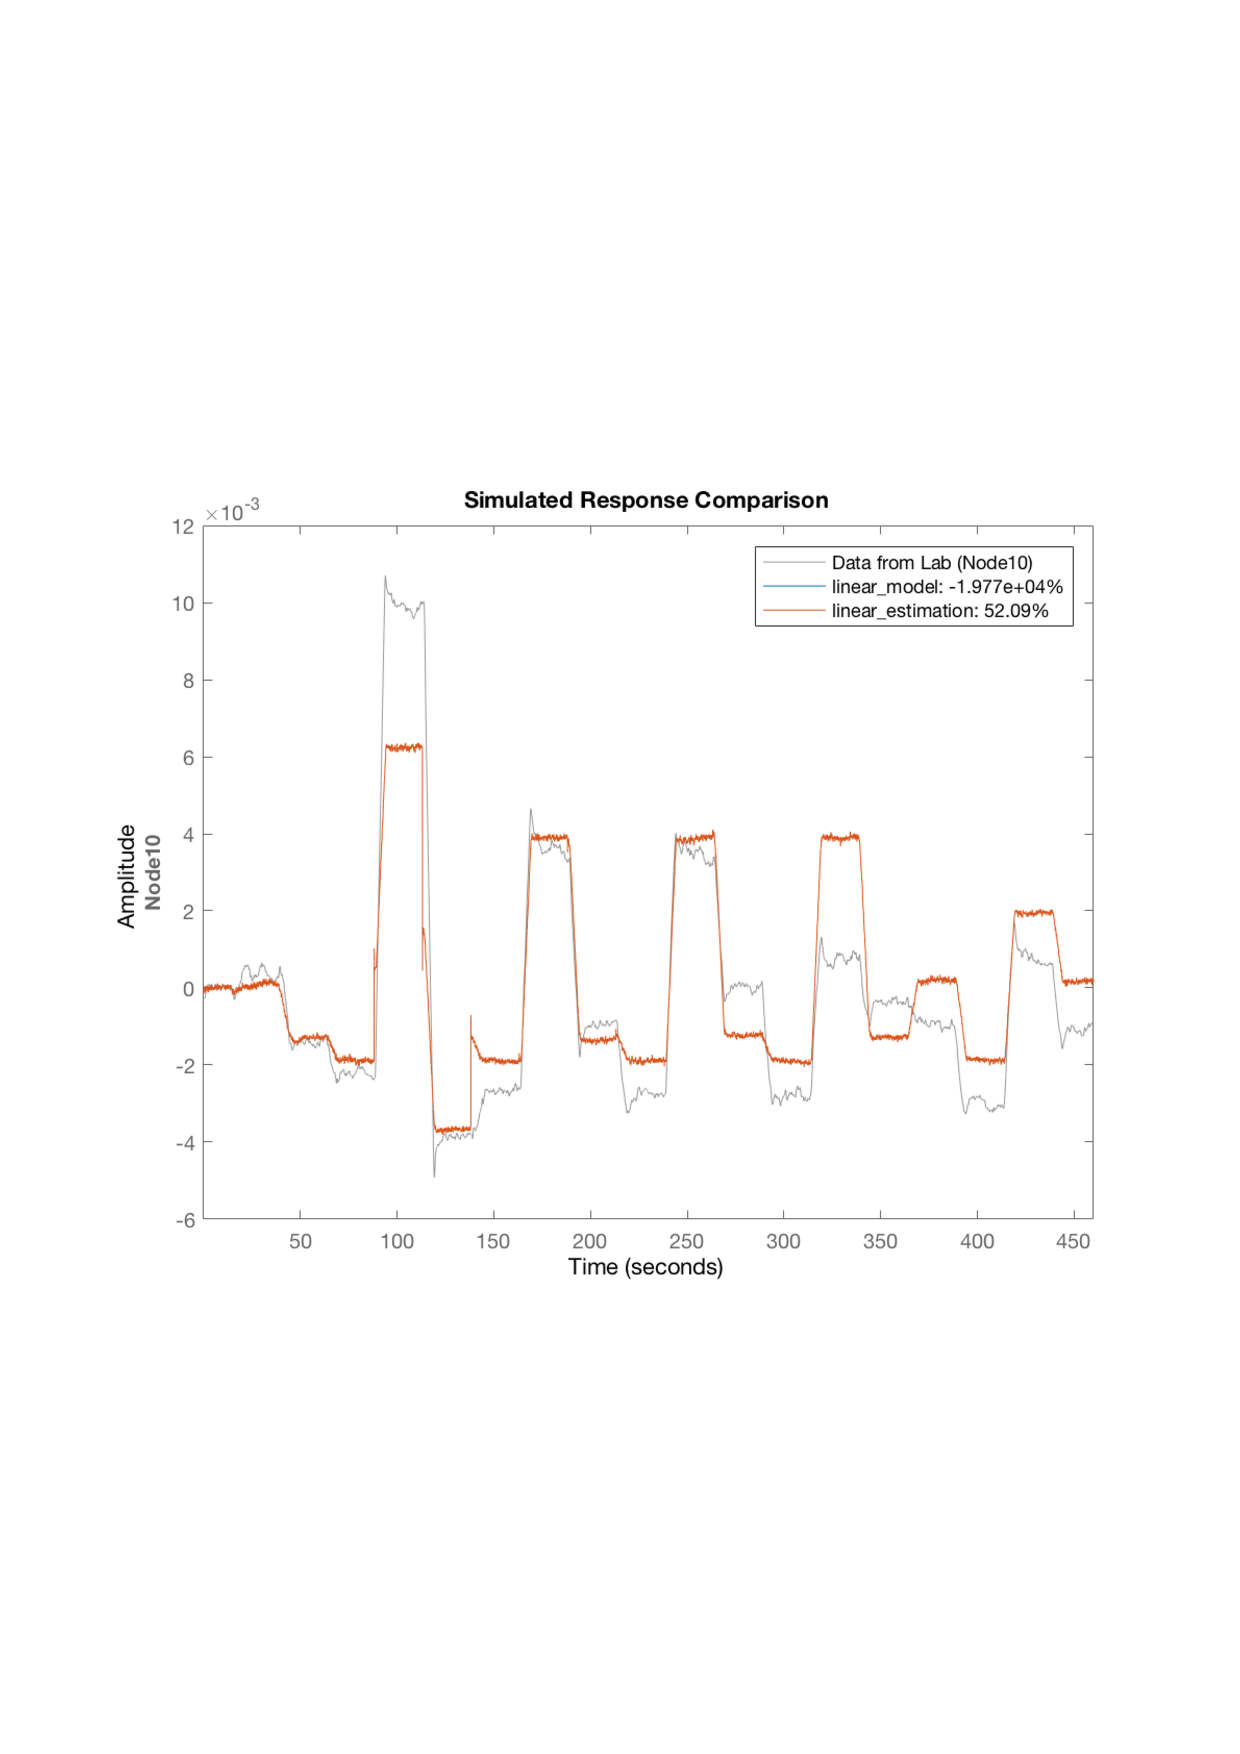
\includegraphics[width=\textwidth]{report/pictures/Node10_estimation.pdf}
    \caption{Estimation comparison for node 10.}
  \end{minipage}
  \hfill
  \begin{minipage}[b]{0.45\textwidth}
    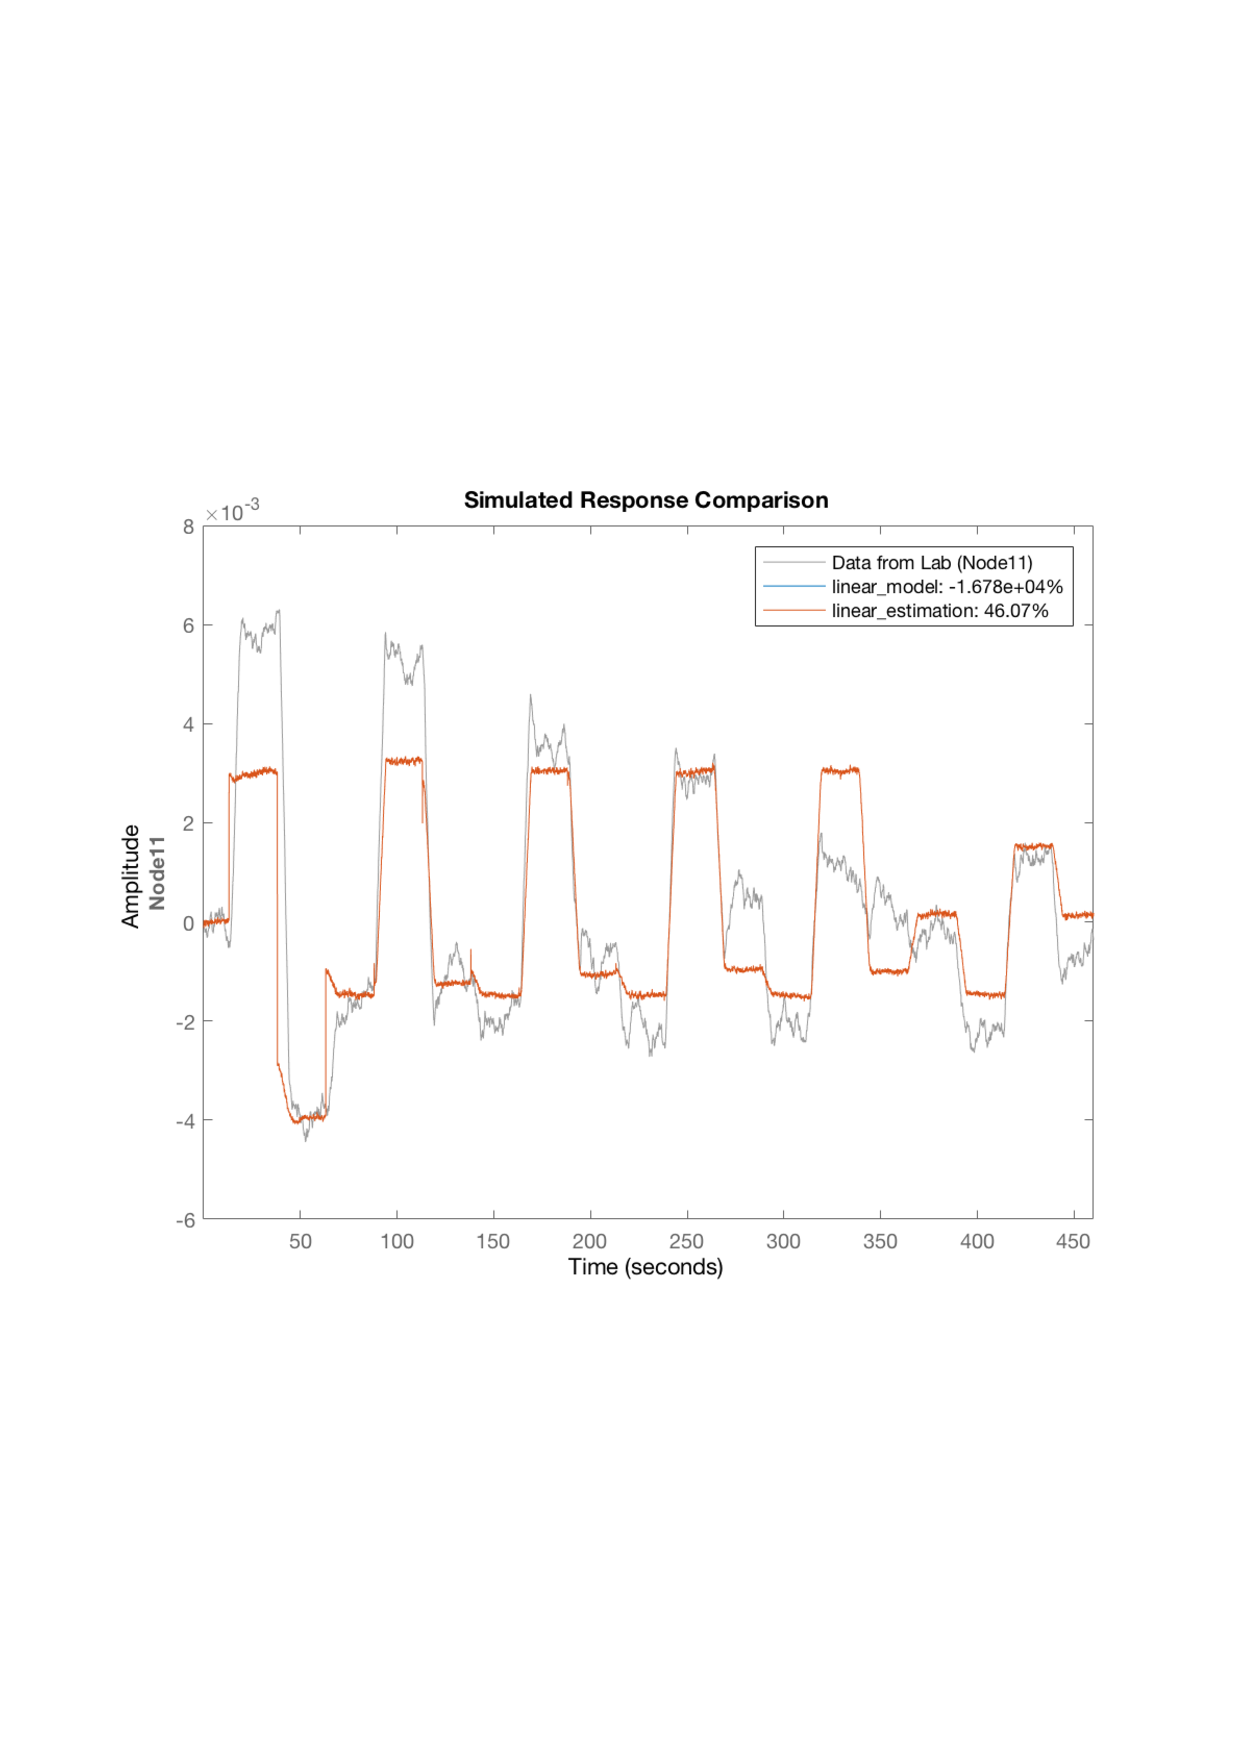
\includegraphics[width=\textwidth]{report/pictures/Node11_estimation.pdf}
    \caption{Estimation comparison for node 11.}
  \end{minipage}
\end{figure}

\begin{figure}[H]
  \centering
  \begin{minipage}[b]{0.45\textwidth}
    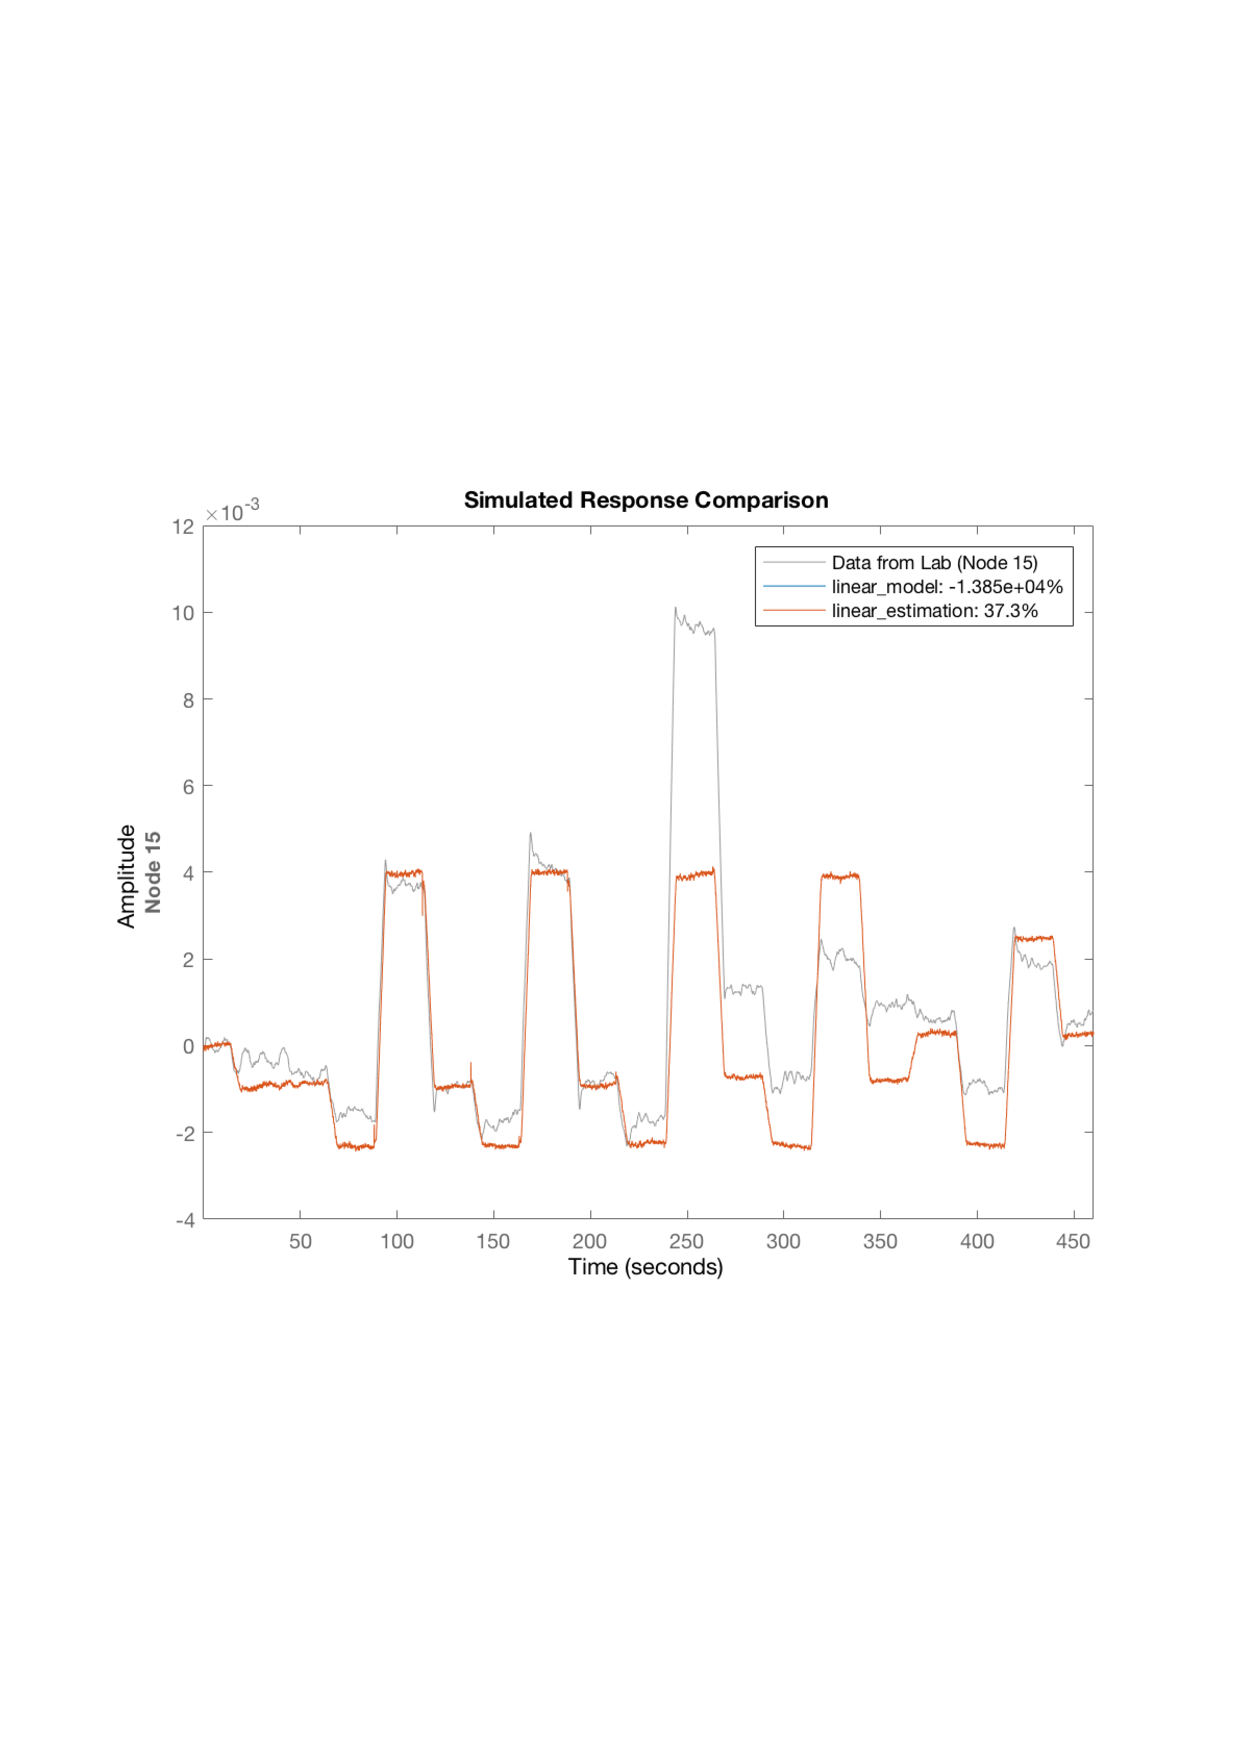
\includegraphics[width=\textwidth]{report/pictures/Node15_estimation.pdf}
    \caption{Estimation comparison for node 15.}
  \end{minipage}
  \hfill
  \begin{minipage}[b]{0.45\textwidth}
    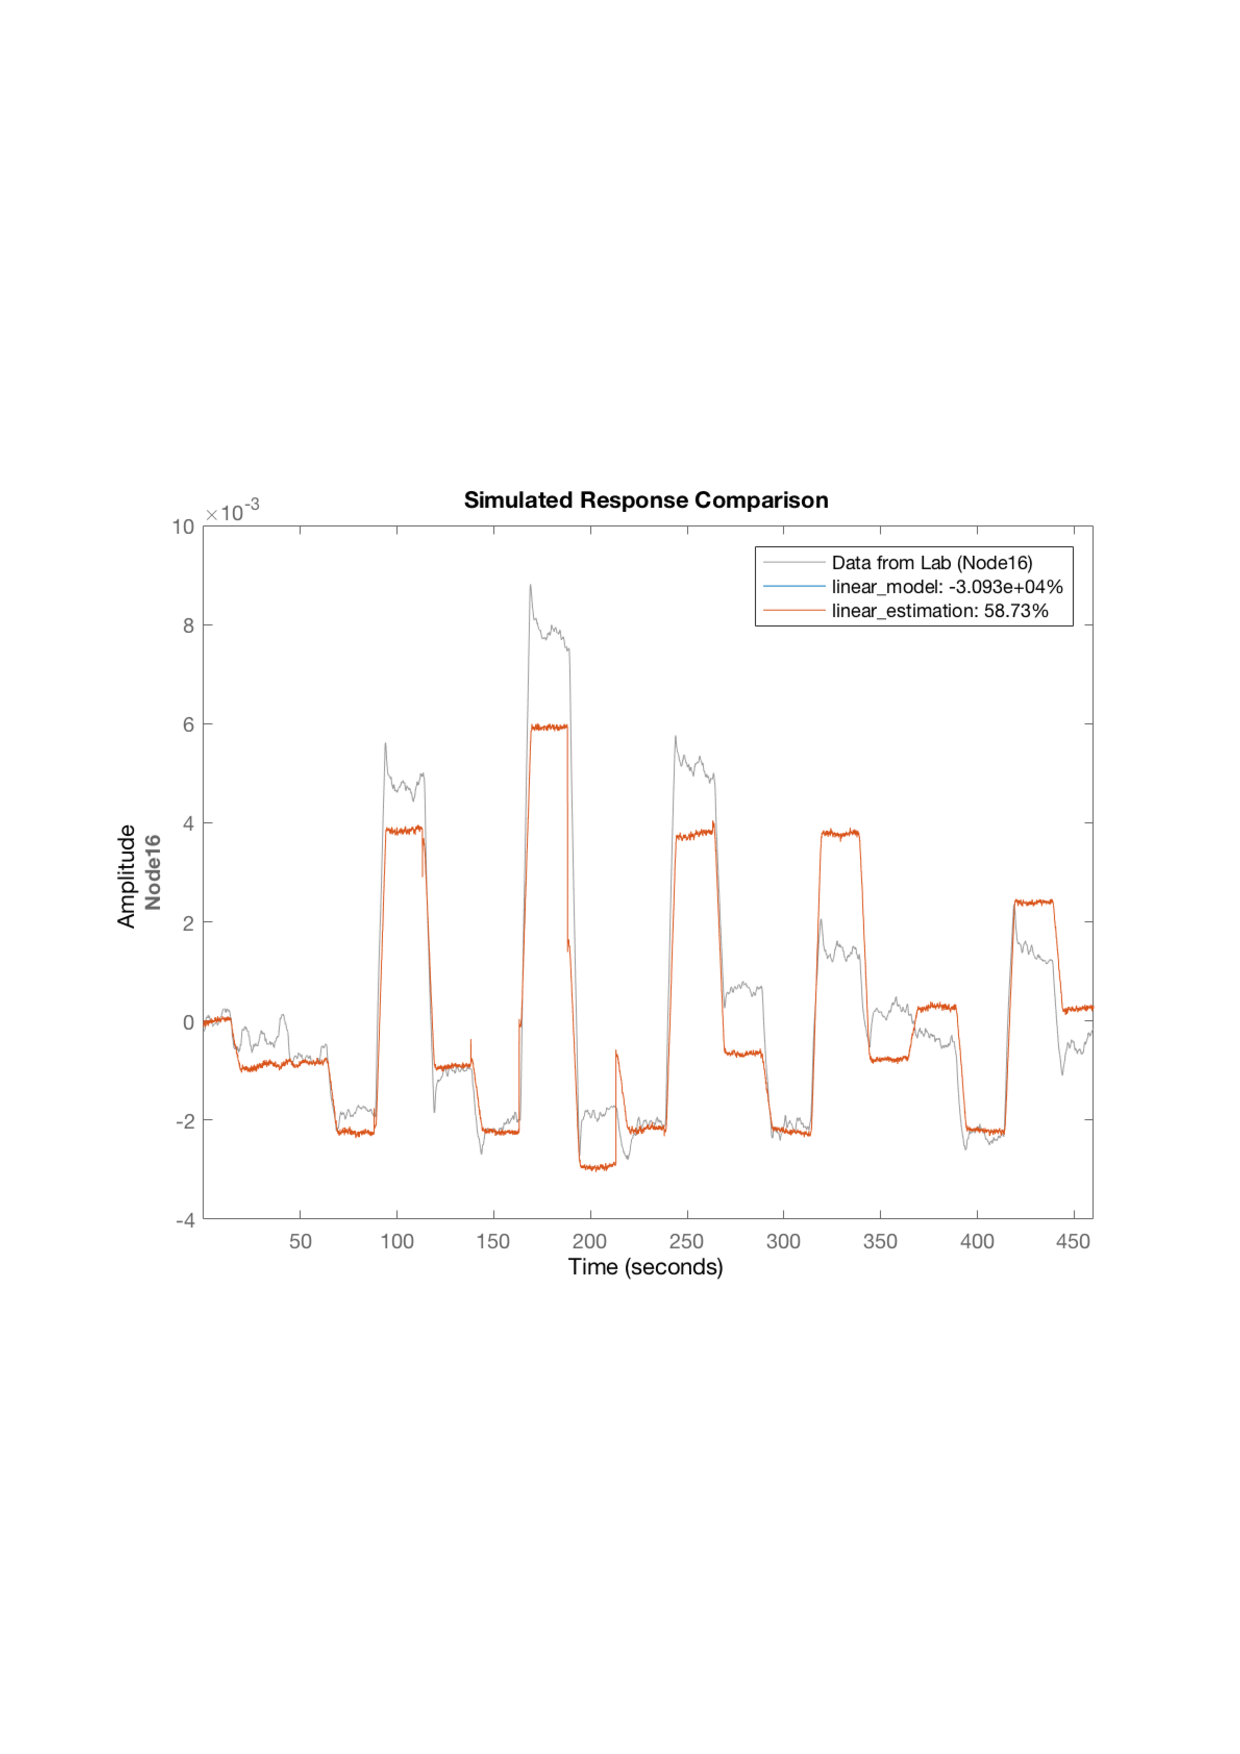
\includegraphics[width=\textwidth]{report/pictures/Node16_estimation.pdf}
    \caption{Estimation comparison for node 16.}
  \end{minipage}
\end{figure}

\begin{figure}[H]
 \centering
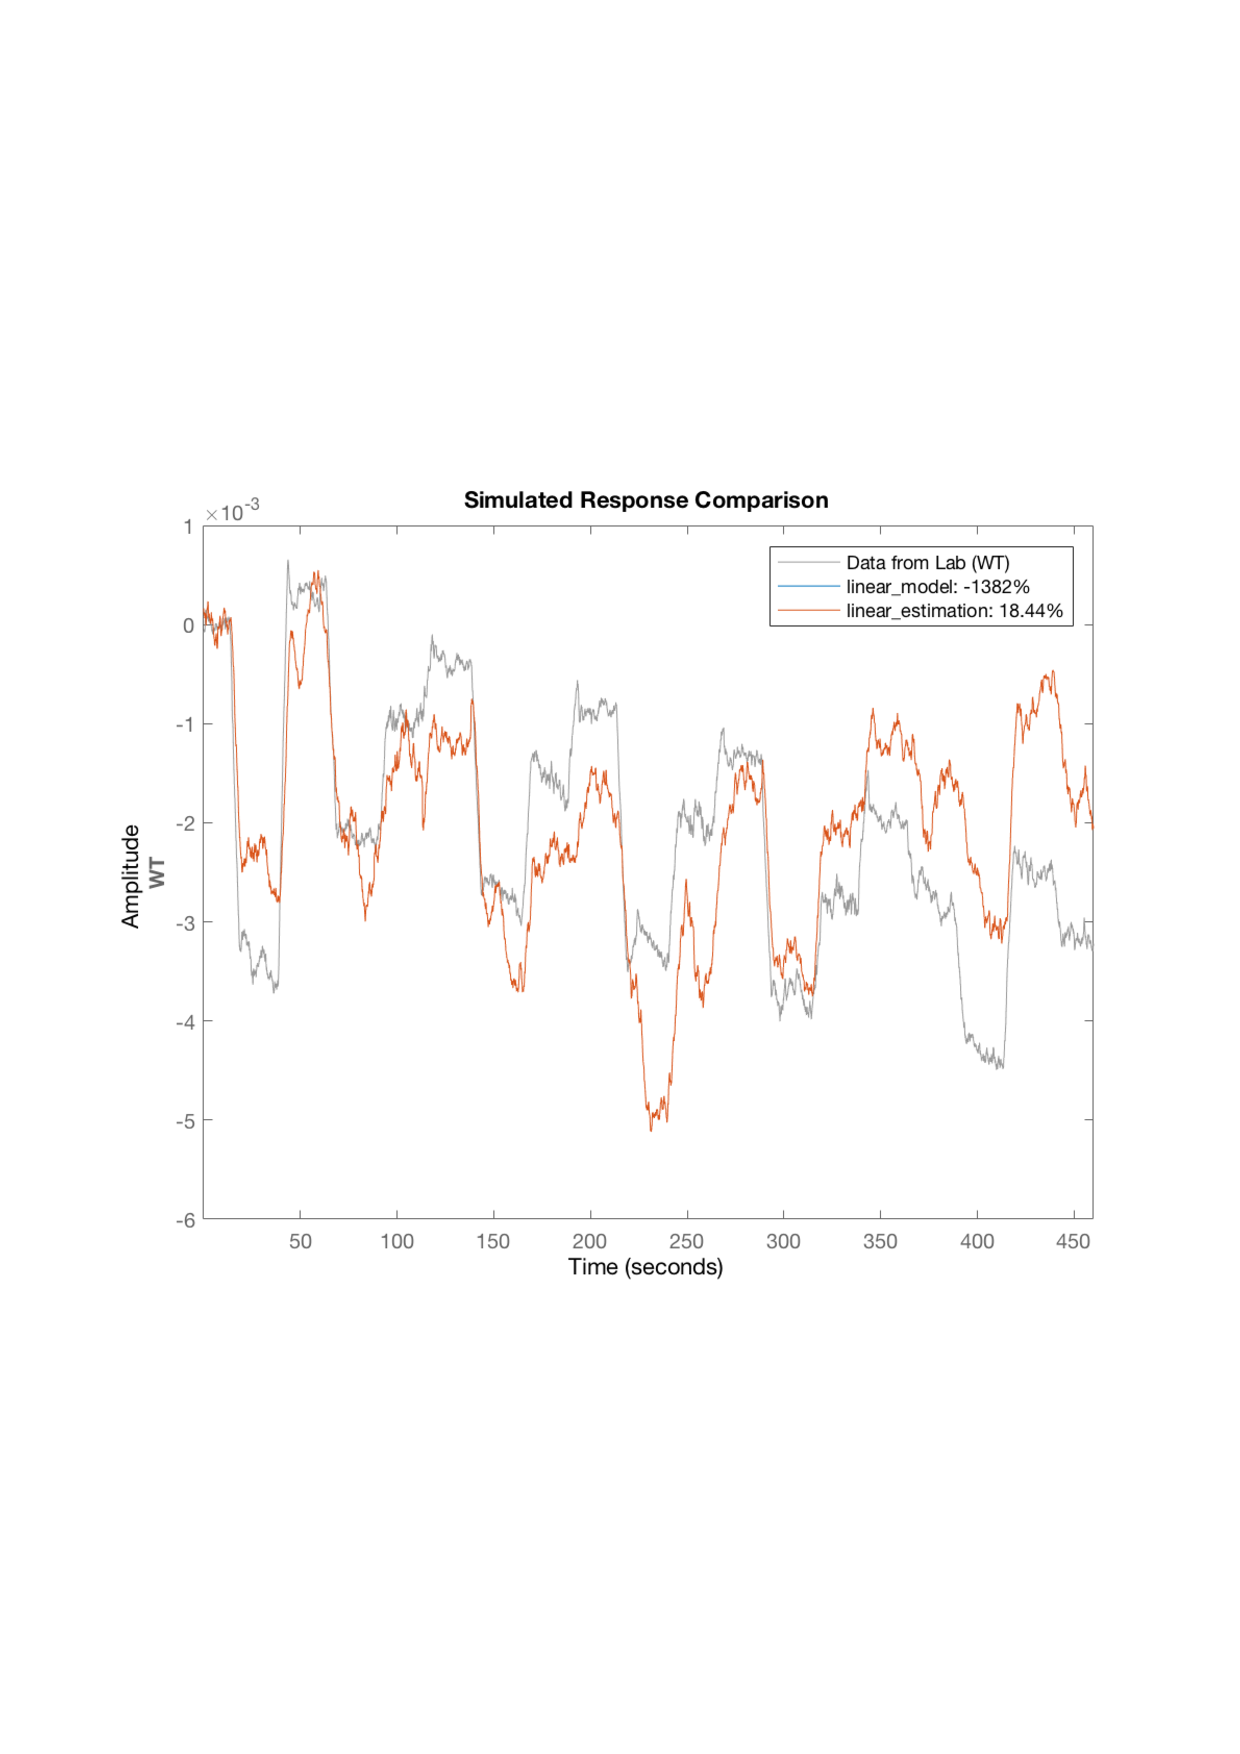
\includegraphics[scale=0.45]{report/pictures/WT_estimation.pdf}
    \caption{Estimation comparison for WT.}
\end{figure}
